\documentclass[a4paper]{article}

\setlength\parindent{0pt}

\usepackage[left=2cm,right=2cm,top=3cm,bottom=3cm,includeheadfoot]{geometry}

\usepackage[utf8x]{inputenc} %soll utf8 als code verwenden
\PrerenderUnicode{äöüÄÖÜß} % umlaute gehen nun auch

\usepackage[ngerman]{babel} % deutsche Bezeichnungen

\usepackage{amssymb} % mathe symbole
\usepackage{amsmath} % mathe formeln
\usepackage{amsthm} % mathe theoreme
\usepackage{graphicx} % Darstellung von Bildern

\usepackage{pstricks}


% - Times, Helvetica, Courier (Word Standard...)
\usepackage{mathptmx}
\usepackage[scaled=.90]{helvet}
\usepackage{courier}
\usepackage{listings}

\newtheorem{lemma}{Lemma}

\usepackage{fancyhdr}
\pagestyle{fancy}



\begin{document}

\lhead{Proseminar\\ Theoretische\\ Informatik}
\chead{Ausarbeitung \\ $\;$ \\}
\rhead{Johannes Honke\\ Marko Jahn\\ Stephan Mielke}

\cfoot{Monotone vs. Non-monotone Circuit Complexity}

$\;$ \\

In einem $U_2$ Schaltkreis gibt es nur Gatter der Form $(x^a\oplus y^b)^c$ enth\"alt,die nur zwei Eing\"anget haben.\\
% Bei einem $U_2$ Schaltkreis handelt es sich um einen Schaltkreis bei dem nur die Gatter AND, OR und NOT mit 2 Eingängen verwendet werden.\\

\begin{lemma}
  Gegeben ist ein beliebiger $U_2$ Schaltkreis $\beta$. F\"ur diesen gibt es einen Schaltkreis $\beta’$, der h\"ochstens
  die zweifache Gr\"o\ss{}enkomplexit\"at hat wie $\beta$. In $\beta’$ wurden alle Verneinungen entfernt und f\"ur jeden Eing\"ange von
  $\beta$ wird auch sein Inverses bereit gestellt.
% Für jeden $U_2$ Schaltkreis $\beta$, gibt es einen äquivalnten Schaltkreis, welcher höchstens
% 2 mal so groß ist wie $\beta$, in dem nur NOT-Gatter nur bei den Variablen benutzt werden.
\end{lemma}

$\forall \; \beta \in U_2 \; \exists \; \beta' : C(\beta') \leq 2 \cdot C(\beta)$\\

Gucken wir uns zuerst die Gatter nochmal genauer an. Wir haben die Gatter der Form $(x^a\oplus y^b)^c$, wobei $\oplus$ die Operation $\wedge$ oder $\vee$ darstellt
und die Variablen $a,b,c \in \{0,1\}$ angeben ob man das Inverse oder die Projektion benutzt. Somit k\"onnen wir sagen das $x^1$ das Inverse und
$x^0$ die Projektion darstellt. Als Operation nehmen wir nun $\wedge$ an (mit $\vee$ ist es analog) so k\"onnen wir folgene Tabelle mit hilfe der Regeln von DeMorgan\footnote{$\overline{a\land{}b}=\overline{a}\lor\overline{b}$} erstellen.\\

\begin{tabular}{|cc|c|c|c|c|}\hline
 $a$    & $b$   & $c = 0$                               & $c = 0$ DeMorgan                              & $c=1$                                                 & $c = 0$ DeMorgan\\
  0     & 0     & $(x \wedge y)$                        & $\overline{(\overline{x} \vee \overline{y})}$ & $\overline{(x \wedge y)}$                             & $(\overline{x} \vee \overline{y})$ \\
  0     & 1     & $(x \wedge \overline{y})$             & $\overline{(\overline{x} \vee y)}$            & $\overline{(x \wedge \overline{y})}$                  & $(x \vee \overline{y})$ \\
  1     & 0     & $(\overline{x} \wedge y)$             & $\overline{(x \vee \overline{y})}$            & $\overline{(\overline{x} \wedge y)}$                  & $(\overline{x} \vee y)$ \\
  1     & 1     & $(\overline{x} \wedge \overline{y})$  & $\overline{(x \vee y)}$                       & $\overline{(\overline{x} \wedge \overline{y})}$       & $(x \vee y)$ \\ \hline
\end{tabular}\\

Mit dieser Tabelle stellen wir einen beliebigen $U_2$ Schaltkreis um sodass er das Lemma erf\"ullt.
Wir beginnen am Ausgang (Top) und arbeiten uns zu dein Eing\"angen (Bottom) (Top-Down-Prinzip) und erstellen f\"ur jedes Gatter $z = (x^a\oplus y^b)^c$ zwei neue Gatter
$z_0, z_1$ wobei $z_0 = (x^a\oplus y^b)^0$ und $z_1 =  (x^a\oplus y^b)^1$ repr\"asentieren. Somit haben wir f\"ur jedes Gatter die Projektion und das Inverse in unserem neuen Schaltkreis.
Dieser Schaltkreis hat eine Gr\"o\ss{}enkomplexit\"at von dem zweifachen der Gr\"o\ss{}enkomplexit\"at unseres alten Schaltkreises und erf\"ullt somit das Lemma indem wir alle Vermeinungen entfernt haben.\\

Am Ende k\"onnen wir noch alle \"uberfl\"ussigen Gatter entfernen von denen der Ausgang nicht abh\"angig ist. \\

\qed{}





% Um das zu erreichen gehen wir von Oben (dem Ausgang) nach Unten (den Eing\"angen), also nach dem Top-Down Prinzip vor.
% Wir stellen f\"ur jedes Gatter auch sein Inverses zu Verf\"ugung. Aus $z^c = (x^a \wedge y^b)$ wird, $z = (x \wedge y)$ und $\overline{z} = (\overline{x} \vee \overline{y})$
% nach den Regeln von deMorgan\footnote{$\overline{a\land{}b}=\overline{a}\lor\overline{b}$}. Analog gilt das auch f\"ur $\vee$.
% Somit hat der neue Schaltkreis die dopplete Komplexit\"at vom alten. Den neuen Schaltkreis k\"onnen wir weiter Optimieren in dem wir nicht ben\"otigte Gatter wieder entfernen.\\
% z.B.: den zweiten Ausgang sowie alle anderen Gatter die ins \glqq Nichts\textquotedblright $\;$ f\"uhren.\\
% Am Ende erhalten wir den gew\"unschten aquivalenten $\beta'$ f\"ur $\beta$.\\

% Als erstes werden die Gatter topologisch sortiert. Also Gatter die andere Gatter an ihren Eingängen haben kommen nach diesen.
% Nun beginnen wir mit dem obersten Gatter. Sollte dessen Ausgang verneint sein, so wenden wir darauf die Regel von deMorgan\footnote{$\overline{a\land{}b}=\overline{a}\lor\overline{b}$ Analog für OR} an.
% Sollten die Ausgänge verneint sein so verschieben wir diese Verneinung auf die Ausgänge der vorhergehenden Gatter, wobei sich doppelte Verneinungen Aufheben.
% Dies wird wiederholt für alle vorhergehenden Gatter.
% Für den Fall, dass ein Gatter negiert und nicht negiert verwendet wird, wird dieses Gatter verdoppelt.\\
% \qed{}

Nun folgt ein Beispiel: \\

Wir nehmen uns die Funktion: $x_{out} = (x_1 \oplus (\overline{x_2} \oplus (x_3 \wedge \overline{x_4})))$ und
stellen daf\"ur den entsprechenden $U_2$ Schaltkreis auf, Dieser hat eine Gr\"o\ss{}enkomplexit\"at von 7.\\

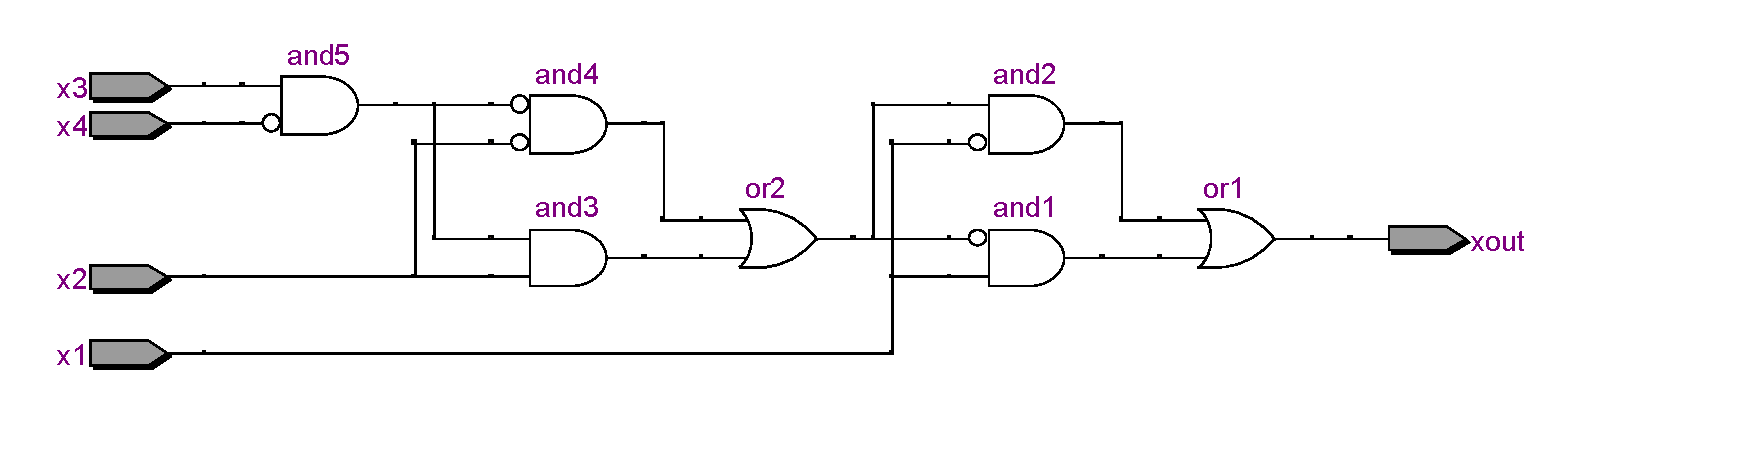
\includegraphics[scale=0.50]{images/ursk.pdf}

Nun gehen wir wie oben beschrieben nach dem Top-Down-Prinzip durch und stellen in unserem neuen Schaltkreis f\"ur jedes Gatter
die Projektion und sein Inverses bereit. Hierbei k\"onnen \"aquivalente Teilschaltkreise entstehen, die wir wieder zusammenfassen k\"onnen.
Unser neuer Schaltkreis hat eine Gr\"o\ss{}enkomplexitvon 14 also $7 * 2 = 14$ somit erf\"ullt er das Lemma. \\


% Nun stellen wir f\"ur jedes Gatter vom Ende aus auch sein Inverses bereit nach der Regel von deMorgan, bis wir bei
% den Inputs angekommen sind. F\"ur jedes der Inputs stellen wir nun auch das Inverse bereit und verkn\"upfen diese mit den Gattern.
% Bei diesem Schritt k\"onnen \"aquivalente Teilschaltkreise entstehen, die wir wieder zusammen fassen k\"onnen, sodass wir eine Komplexit\"at von 14 erreichen.
% Somit erhalten wir den folgenen Schaltkreis.\\

% Dieser Schaltkreis ist um $U_2$ so wie es das Lemma bereits verlangt.
% Es hat eine $C(s) = 7$ dem zu folge sollte der neue Schaltkreis maximal eine von $14$ haben.
% Zu erst stellen wir zu jedem Input auch sein Inverses bereit und von oben nach Unten (top down) stellen wir nun
% f\"ur jedes Gatter auch sein Inverses nach den Regeln von DeMorgan zu verf\"ugung.
% Bei diesem Schritt kann es dazu kommen das wir zwei \"aquivalente Teilschaltkreise bekommen die wir zusammen f\"ugen k\"onnen. \\

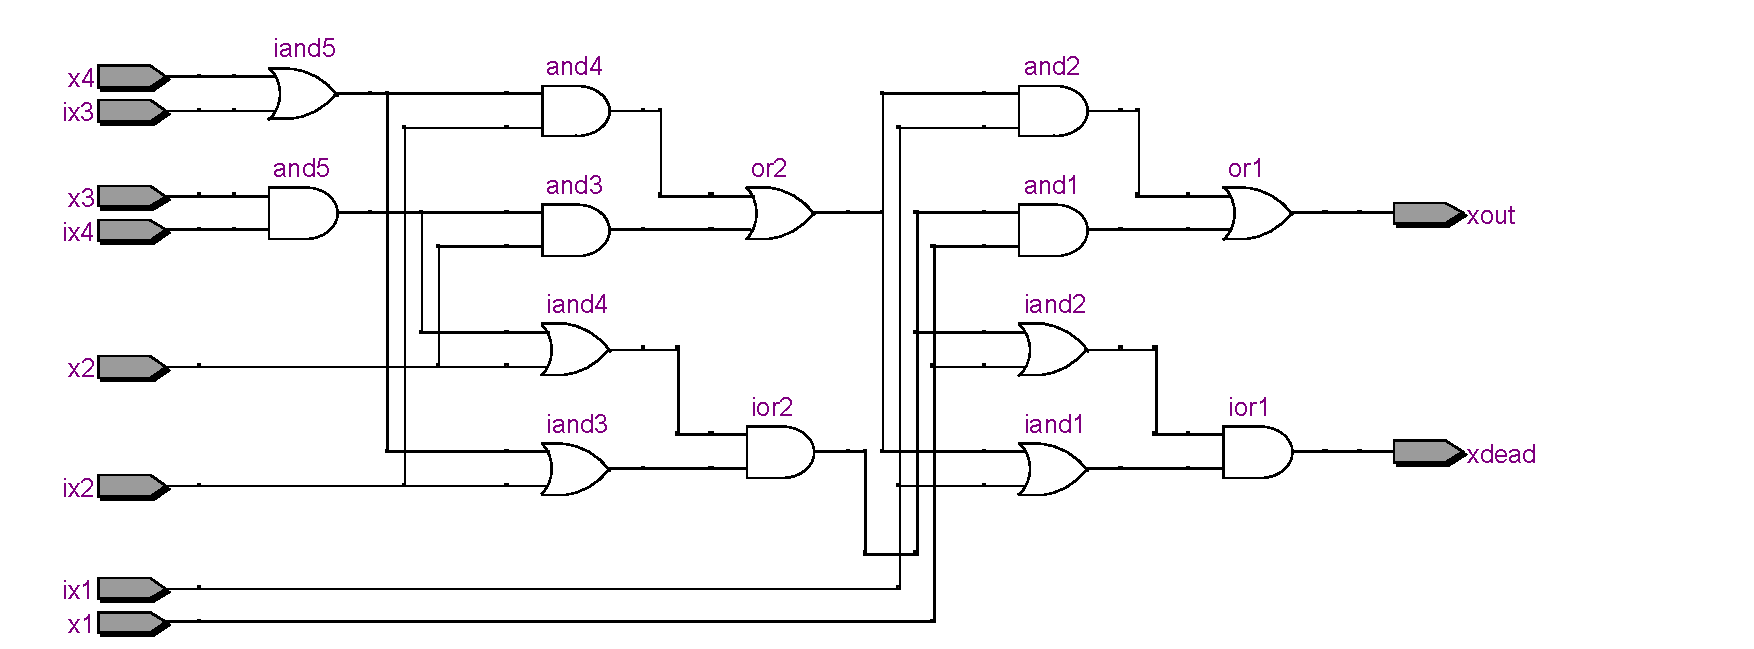
\includegraphics[scale=0.50]{images/zwisk.pdf}

Am Ende konnten wir noch \"uberfl\"ussige Gatter entfernen, weil von ihnen der Ausgang nicht abh\"angig war und erreichen das unser Schaltkreis sogar kleiner
als 14 geworden ist, n\"amlich 11.\\

% Jetzt k\"onnen wir alle \glqq toten\textquotedblright $\;$Gatter entfernen um den Schaltkreis zu optimieren und erreichen eine Komplexit\"at von 11.\\

% Dieser neue Schaltkreis hat nun eine Komplexit\"at von $14$, also h\"alt er sich an das Lemma. Die Not-Gatter sind auch alle verschwunden und werden nun \"uber
% die Inversen Inputs realisiert. Zum Schluss k\"onnen wir noch \glqq M\"ull\grqq entfernen. Also tote Gatter die wir nicht ben\"otigen da ihre Signale ins Nirvana verschwinden.\\

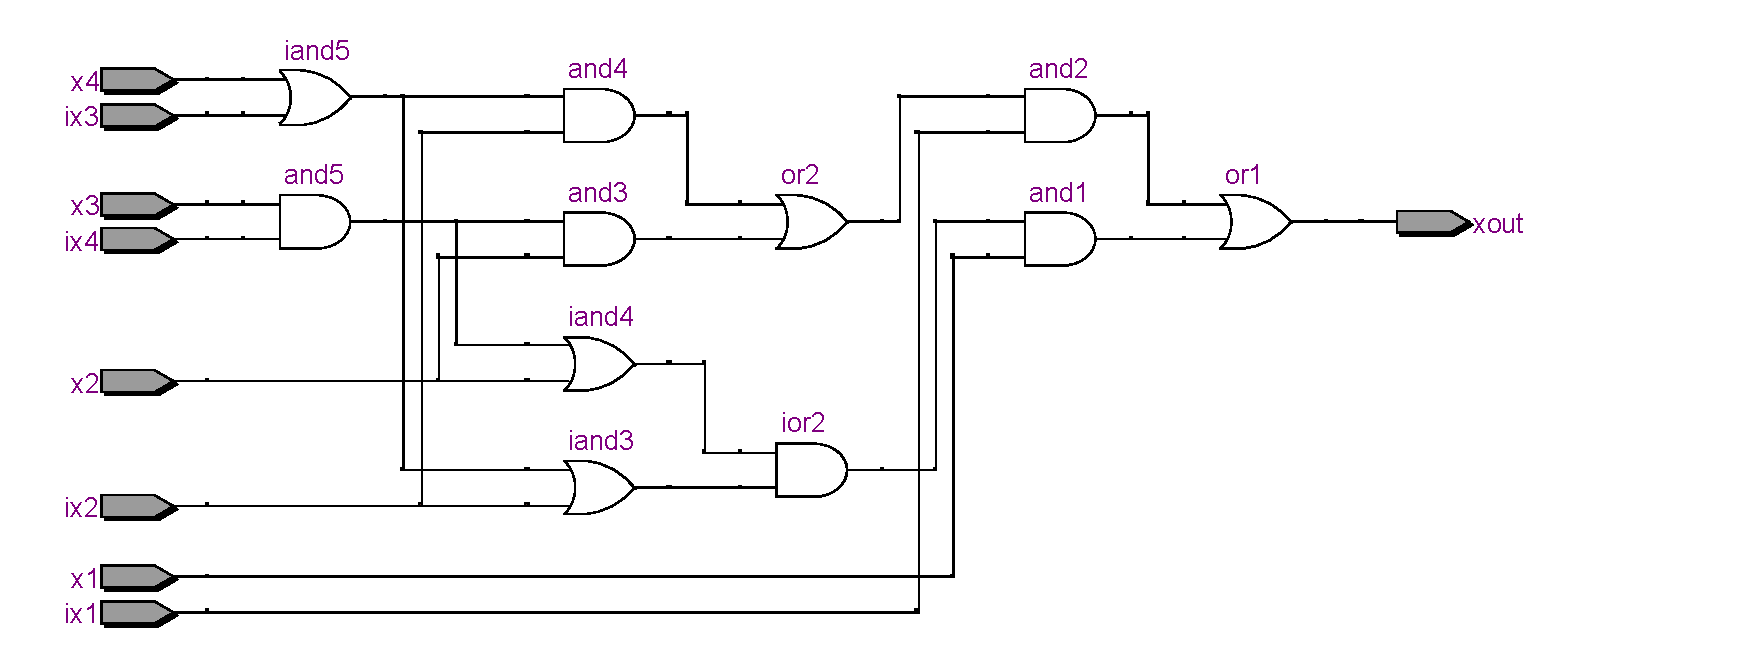
\includegraphics[scale=0.50]{images/endsk.pdf}

% Am Ende konnten wir wieder 3 Gatter entfernen und konnten somit den Schaltkreis optimieren. Die neue Komplexit\"at ist nun $11$ und damit ist diese geringer als das Zweifache der Komplexit\"at des Urschaltkreises.


\end{document}